% Coherence Without Content -- 10-minute sprint talk.
% Build:  latexmk -pdf slides.tex   (or `make slides` in paper/)
%
% Shares numbers.tex and figs/ with main.tex, so the talk cannot quote a
% different number from the paper. Same reason the paper has no typed results.
%
% Timing: ~10 min. Slides 3-6 are the spine; if you are cut short, the talk
% still lands after slide 6 (the scale ladder). Everything after is support.

\documentclass[aspectratio=169,11pt]{beamer}

\usetheme{default}
\usecolortheme{seahorse}
\setbeamertemplate{navigation symbols}{}
\setbeamertemplate{footline}[frame number]
\setbeamercolor{frametitle}{fg=black}
\setbeamerfont{frametitle}{size=\large,series=\bfseries}
\setbeamertemplate{itemize item}{--}
\setbeamertemplate{itemize subitem}{--}

\usepackage[utf8]{inputenc}
\usepackage[T1]{fontenc}
\usepackage{lmodern}
\usepackage{booktabs}
\usepackage{graphicx}
\usepackage{amsmath}

\graphicspath{{figs/}}
% Generated by scripts/paper_numbers.py. Do not edit.
% Every result in main.tex resolves through these macros.
\newcommand{\NModels}{9}
\newcommand{\NCells}{81}
\newcommand{\NSplits}{5}
\newcommand{\MeanR}{0.906}
\newcommand{\MeanFloor}{0.880}
\newcommand{\MeanResidual}{+0.025}
\newcommand{\NClears}{6}
\newcommand{\NNegative}{2}
\newcommand{\BatterySHA}{342db046213099ad}
\newcommand{\MeanDecisiveR}{41}
\newcommand{\MeanDecisiveN}{4.5}
\newcommand{\MedianDecisiveRatio}{17}
\newcommand{\SmolLMThreeThreeBR}{0.938}
\newcommand{\SmolLMThreeThreeBN}{0.929}
\newcommand{\SmolLMThreeThreeBResid}{+0.009}
\newcommand{\SmolLMThreeThreeBFloor}{0.029}
\newcommand{\QwenThreeFiveNineBR}{0.919}
\newcommand{\QwenThreeFiveNineBN}{0.923}
\newcommand{\QwenThreeFiveNineBResid}{-0.004}
\newcommand{\QwenThreeFiveNineBFloor}{0.010}
\newcommand{\LFMTwoFiveOneTwoBInstructR}{0.905}
\newcommand{\LFMTwoFiveOneTwoBInstructN}{0.858}
\newcommand{\LFMTwoFiveOneTwoBInstructResid}{+0.047}
\newcommand{\LFMTwoFiveOneTwoBInstructFloor}{0.023}
\newcommand{\QwenThreeFiveZeroEightBR}{0.904}
\newcommand{\QwenThreeFiveZeroEightBN}{0.838}
\newcommand{\QwenThreeFiveZeroEightBResid}{+0.067}
\newcommand{\QwenThreeFiveZeroEightBFloor}{0.023}
\newcommand{\QwenThreeFiveFourBR}{0.903}
\newcommand{\QwenThreeFiveFourBN}{0.916}
\newcommand{\QwenThreeFiveFourBResid}{-0.013}
\newcommand{\QwenThreeFiveFourBFloor}{0.015}
\newcommand{\gemmaFourETwoBitR}{0.902}
\newcommand{\gemmaFourETwoBitN}{0.892}
\newcommand{\gemmaFourETwoBitResid}{+0.010}
\newcommand{\gemmaFourETwoBitFloor}{0.007}
\newcommand{\graniteFourOneThreebR}{0.896}
\newcommand{\graniteFourOneThreebN}{0.832}
\newcommand{\graniteFourOneThreebResid}{+0.063}
\newcommand{\graniteFourOneThreebFloor}{0.029}
\newcommand{\QwenThreeFiveTwoBR}{0.895}
\newcommand{\QwenThreeFiveTwoBN}{0.892}
\newcommand{\QwenThreeFiveTwoBResid}{+0.003}
\newcommand{\QwenThreeFiveTwoBFloor}{0.001}
\newcommand{\SmolLMTwoOneSevenBInstructR}{0.890}
\newcommand{\SmolLMTwoOneSevenBInstructN}{0.843}
\newcommand{\SmolLMTwoOneSevenBInstructResid}{+0.047}
\newcommand{\SmolLMTwoOneSevenBInstructFloor}{0.015}
\newcommand{\LadderSmall}{Qwen3.5-0.8B}
\newcommand{\LadderLarge}{Qwen3.5-9B}
\newcommand{\LadderRRise}{+0.014}
\newcommand{\LadderNRise}{+0.085}
\newcommand{\LadderResidFall}{-0.071}
\newcommand{\PooledSizeCorr}{-0.67}
\newcommand{\PooledFloorCorr}{+0.68}
\newcommand{\LadderFamily}{qwen}
\newcommand{\LadderNSizes}{4}
\newcommand{\WithinFamilyCorr}{-0.84}
\newcommand{\OutsideFamilyCorr}{-0.19}
\newcommand{\NOutsideFamily}{5}
\newcommand{\TokensR}{13.2}
\newcommand{\TokensNm}{26.6}
\newcommand{\TokenInflation}{2.0}
\newcommand{\MatchedBandLo}{13}
\newcommand{\MatchedBandHi}{24}
\newcommand{\MatchedResidual}{+0.021}
\newcommand{\RealLengthRule}{0.541}
\newcommand{\RealTiedAcc}{0.899}
\newcommand{\RealDecompFit}{0.904}
\newcommand{\FloorLengthRule}{0.695}
\newcommand{\FloorTiedAcc}{0.848}
\newcommand{\FloorDecompFit}{0.884}
\newcommand{\MostLengthModel}{granite-4.1-3b}
\newcommand{\MostLengthRule}{0.835}
\newcommand{\MostLengthFit}{0.833}
\newcommand{\NMassDrop}{8}
\newcommand{\MedianMassDrop}{+0.011}
\newcommand{\MassDropSignP}{0.039}
\newcommand{\ReasoningModel}{SmolLM3-3B}
\newcommand{\ReasoningMassDrop}{0.193}
\newcommand{\ReasoningResid}{+0.009}
\newcommand{\MassDropExclReasoning}{+0.009}
\newcommand{\ResidShiftAnswered}{+0.002}
\newcommand{\PersonaSignCorrect}{20}
\newcommand{\PersonaSignTotal}{20}
\newcommand{\PersonaSepReal}{+0.791}
\newcommand{\PersonaSepInvented}{+0.781}
\newcommand{\PersonaExcess}{+0.133}
\newcommand{\PersonaNonsenseShare}{66}
\newcommand{\PersonaNRetain}{2}
\newcommand{\PersonaNModelsTested}{5}
\newcommand{\PersonaRetainTop}{Qwen3.5-9B}
\newcommand{\PersonaRetainTopVal}{+0.415}
\newcommand{\DetKeptAuroc}{0.596}
\newcommand{\DetKeptTPR}{0}
\newcommand{\DetBestName}{answer mass}
\newcommand{\DetBestAuroc}{0.821}
\newcommand{\DetBestTPR}{40}
\newcommand{\DetFPR}{5}
\newcommand{\DetNModels}{9}
\newcommand{\DetBestModel}{Qwen3.5-2B}
\newcommand{\DetBestModelAuroc}{1.000}
\newcommand{\StatedNModels}{5}
\newcommand{\StatedNResponsive}{4}
\newcommand{\StatedNItems}{12}
\newcommand{\StatedHaveLo}{0.869}
\newcommand{\StatedHaveHi}{1.000}
\newcommand{\StatedHideLo}{0.901}
\newcommand{\StatedHideHi}{1.000}
\newcommand{\StatedFakeLo}{0.947}
\newcommand{\StatedFakeHi}{0.999}
\newcommand{\StatedBaseLo}{0.246}
\newcommand{\StatedBaseHi}{0.491}
\newcommand{\StatedInertModel}{LFM2.5-1.2B-Instruct}
\newcommand{\StatedInertLo}{0.500}
\newcommand{\StatedInertHi}{0.547}
\newcommand{\StatedInertBase}{0.491}
\newcommand{\StatedNScored}{24}
\newcommand{\StatedWorstModel}{gemma-4-E2B-it}
\newcommand{\StatedWorstCond}{verbal}
\newcommand{\StatedWorstScored}{16}
\newcommand{\StatedWorstMass}{0.67}
\newcommand{\RevNModels}{5}
\newcommand{\RevNTriad}{3}
\newcommand{\RevNInterp}{2}
\newcommand{\RevSpecMargin}{0.30}
\newcommand{\RevGapLo}{+0.054}
\newcommand{\RevGapHi}{+0.059}
\newcommand{\RevSpecLo}{+0.88}
\newcommand{\RevSpecHi}{+1.40}
\newcommand{\RevInertModel}{LFM2.5-1.2B-Instruct}
\newcommand{\RevInertMargin}{+0.116}
\newcommand{\RevInertGap}{-0.041}
\newcommand{\RevDropModel}{gemma-4-E2B-it}
\newcommand{\RevDropPairs}{224}
\newcommand{\RevKeptPairs}{4776}
\newcommand{\RevNInvented}{1}
\newcommand{\RevInventedModel}{Qwen3.5-2B}
\newcommand{\RevInventedConcealed}{+0.890}
\newcommand{\RevInventedVerbal}{+0.635}
\newcommand{\RevInventedGap}{+0.255}
\newcommand{\NeutModel}{Qwen3.5-2B}
\newcommand{\NeutResidBinary}{+0.006}
\newcommand{\NeutResidNeutral}{+0.006}
\newcommand{\NeutFloorShift}{+0.003}
\newcommand{\NeutCohRealBin}{0.896}
\newcommand{\NeutCohRealNeut}{0.898}
\newcommand{\NeutPCReal}{0.316}
\newcommand{\NeutPCPctReal}{32}
\newcommand{\NeutMajReal}{3}
\newcommand{\NeutCohInvBin}{0.889}
\newcommand{\NeutCohInvNeut}{0.892}
\newcommand{\NeutPCInv}{0.638}
\newcommand{\NeutPCPctInv}{64}
\newcommand{\NeutMajInv}{90}
\newcommand{\NPersonaCells}{20}
\newcommand{\NPersonaModels}{5}
\newcommand{\PersonaAbovePointThree}{18}
\newcommand{\PersonaMax}{+0.85}
\newcommand{\PersonaMin}{-0.66}
\newcommand{\DepthSpread}{0.109}
\newcommand{\PersonaSpread}{0.276}


\definecolor{accent}{HTML}{B4453A}
\newcommand{\hl}[1]{\textcolor{accent}{\textbf{#1}}}

\title{Coherence Without Content}
\subtitle{A missing control for emergent value systems in LLMs}
\author{Nullcard}
\institute{\small Apart Research Digital Minds Sprint}
\date{15 August 2026}

\begin{document}

\begin{frame}[plain]
  \titlepage
\end{frame}

% ---------------------------------------------------------------------------
% The hook: state the punchline before the method. A sprint audience decides
% in 40 seconds whether to keep listening.
% ---------------------------------------------------------------------------
\begin{frame}{The one-slide version}
  \Large
  A published metric says these models have coherent values.

  \bigskip
  We ran it on outcomes that \hl{mean nothing}.

  \bigskip
  \begin{center}
  \begin{tabular}{@{}lr@{}}
    real outcomes        & \MeanR{} \\
    meaningless outcomes & \MeanFloor{} \\
    \midrule
    difference           & \hl{\MeanResidual{}} \\
  \end{tabular}
  \end{center}

  \bigskip
  \normalsize
  The metric is not broken. It is \hl{unanchored}.
\end{frame}

\begin{frame}{The claim we are testing}
  \textbf{Utility Engineering} (Mazeika et al., 2025)
  \begin{itemize}
    \item Ask a model to choose between two outcomes, 500 of them
    \item Fit a Thurstonian utility model to the choices
    \item Report held-out accuracy as \emph{structural coherence}
    \item It rises with scale $\Rightarrow$ ``value systems emerge''
  \end{itemize}

  \bigskip
  Their robustness checks vary \emph{how the question is asked}: seven
  languages, syntax, framing, option labels, long context.

  \bigskip
  \begin{center}
  \hl{No condition varies whether the outcomes mean anything.}
  \end{center}
\end{frame}

\begin{frame}{Why that gap is reachable, not pedantic}
  High held-out accuracy proves choices follow a \emph{stable scalar ordering}.
  It does not prove the ordering is \emph{about} anything.

  \bigskip
  \begin{itemize}
    \item \hl{244 of 510 outcomes contain a numeral} --- orderable by
      arithmetic alone. Whole categories are 100\% numeric.
    \item In simulation, a responder ordering purely by magnitude, with
      \hl{zero semantics}, scores \hl{0.949--0.977} held out.
    \item A responder with a genuine latent utility function scores
      0.858--0.928 --- \hl{lower}.
  \end{itemize}

  \bigskip
  An instrument where ``count the number'' beats ``have values'' cannot tell
  them apart from its own output.
\end{frame}

% ---------------------------------------------------------------------------
\begin{frame}{The control}
  Same 510 outcomes. Same prompt, verbatim. Same fit. Same metric.
  \hl{Only the referents change.}

  \bigskip
  \begin{center}
  \begin{tabular}{@{}lll@{}}
    \toprule
    arm & outcomes & coherence would reflect \\
    \midrule
    \textbf{R}                  & real & values $+$ arithmetic $+$ format \\
    \textbf{N\textsuperscript{+}} & invented, magnitudes kept & arithmetic $+$ format \\
    \textbf{N\textsuperscript{--}} & invented, magnitudes gone & \hl{format alone} \\
    \bottomrule
  \end{tabular}
  \end{center}

  \bigskip
  \textbf{N\textsuperscript{--}} is the floor: what the procedure returns when
  there is nothing to have a preference \emph{about}.

  \medskip
  \small Every number we report is $\mathbf{R} - \mathbf{N^{-}}$, never a raw
  coherence. \NModels{} models, \NCells{} cells, 3 design replicates each.
\end{frame}

\begin{frame}{Result 1 --- the metric barely notices}
  \begin{center}
    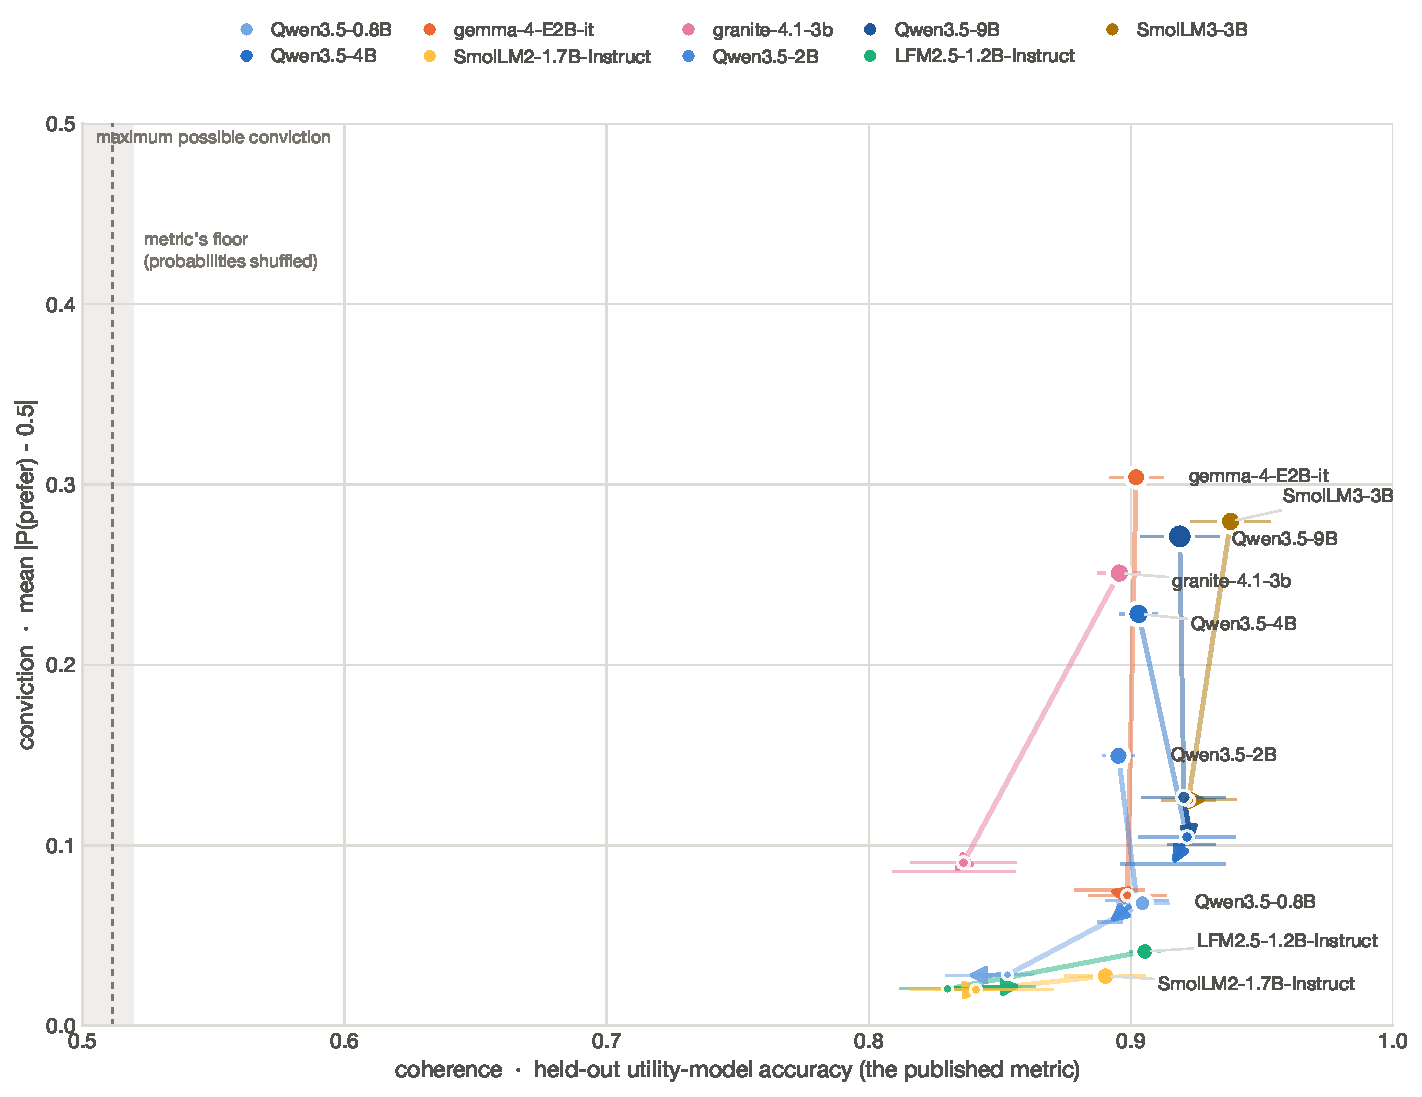
\includegraphics[height=.62\textheight,width=\textwidth,keepaspectratio]{fig1_state_space.pdf}
  \end{center}
  \small
  Each model is a \emph{path}: real $\rightarrow$ invented-with-magnitudes
  $\rightarrow$ invented. If the metric tracked meaning, paths would run
  down-\emph{and-left}. They run \hl{almost straight down}.
\end{frame}

\begin{frame}{Result 2 --- direction survives, conviction does not}
  The metric thresholds preferences to hard labels.
  A pair at $p=0.51$ counts exactly like a pair at $p=0.99$.

  \bigskip
  \begin{center}
  \begin{tabular}{@{}lr@{}}
    \toprule
    commits to a side, real outcomes      & \MeanDecisiveR\% \\
    commits to a side, invented outcomes  & \MeanDecisiveN\% \\
    \midrule
    median collapse                        & \hl{\MedianDecisiveRatio$\times$} \\
    \bottomrule
  \end{tabular}
  \end{center}

  \bigskip
  A model that is almost perfectly \hl{indifferent about gibberish} --- but
  consistently so --- scores as coherent about it.
\end{frame}

% ---------------------------------------------------------------------------
% The decisive slide. Pre-registered, and it went the way that undercuts the
% scaling claim. Do not rush this one.
% ---------------------------------------------------------------------------
\begin{frame}{Result 3 --- the scaling claim, floor-corrected}
  \textbf{Pre-registered decisive test.} One family, size the only variable,
  \LadderSmall{} $\rightarrow$ \LadderLarge{}.

  \bigskip
  \begin{itemize}
    \item If values emerge with scale: floor stays flat, signal rises.
    \item If it is general answer-consistency: \hl{the floor rises too}.
  \end{itemize}

  \bigskip
  \begin{center}
  \begin{tabular}{@{}lr@{}}
    \toprule
    real-outcome coherence rises by  & \LadderRRise{} \\
    the \hl{floor} rises by           & \hl{\LadderNRise{}} \\
    \midrule
    floor-corrected residual         & \hl{\LadderResidFall{}} \\
    \bottomrule
  \end{tabular}
  \end{center}

  \bigskip
  Bigger models here are not more coherent \emph{about the outcomes}.
  They are more consistent in general.

  \medskip
  \footnotesize
  Pooled over all \NModels{} models $r=\PooledSizeCorr$ ($p=0.043$) --- but that
  is \emph{carried by this family} (within \LadderNSizes{} sizes:
  \WithinFamilyCorr; the other \NOutsideFamily{} models: \OutsideFamilyCorr).
  \hl{We claim it within one family only.}
\end{frame}

\begin{frame}{``Maybe your instrument just can't see anything''}
  Fair objection. So: install a persona and measure the shift on \hl{both arms}.

  \bigskip
  \[
    1 - \frac{\lVert \Delta_{\text{invented}} \rVert}{\lVert \Delta_{\text{real}} \rVert}
    \qquad
    \begin{array}{l}
      1.0 = \text{pure preference change} \\
      0.0 = \text{pure style change}
    \end{array}
  \]

  \bigskip
  \begin{itemize}
    \item \hl{\PersonaAbovePointThree{} of \NPersonaCells{}} conditions exceed
      $+0.30$, up to \PersonaMax{}
    \item One informative exception at \PersonaMin{} --- moved \emph{gibberish}
      further than substance. That is what style looks like.
    \item \hl{Depth barely matters}: user turn vs.\ system prompt shifts it
      \DepthSpread{}; swapping the trait shifts it \PersonaSpread{}
  \end{itemize}

  \bigskip
  So the instrument \emph{can} see content. It is the unmanipulated coherence
  number that fails to depend on it.
\end{frame}

\begin{frame}{Three checks that came out in their favour}
  We report these regardless. They \hl{narrow} our claim.

  \bigskip
  \begin{enumerate}
    \item \textbf{Order effects are handled.} Pure positional bias produces
      exactly 50/50 on counterbalanced pairs. It cancels completely.
    \item \textbf{Not inflated by overfitting.} Held-out evaluation keeps a
      coin flip at 0.46--0.49. \emph{Our first draft claimed otherwise and was
      wrong.}
    \item \textbf{The fit is sound.} Shuffle probabilities across pairs and the
      metric lands at $\sim$0.50.
  \end{enumerate}

  \bigskip
  \begin{center}
  We are not saying the metric is broken.\\
  We are saying \hl{a high score does not distinguish values from format}.
  \end{center}
\end{frame}

\begin{frame}{What we would want you to hold against us}
  \begin{itemize}
    \item \textbf{Tokenisation is not matched --- so we tested it.} Invented
      outcomes carry \TokenInflation$\times$ the tokens. Matched on tokens
      (\MatchedBandLo--\MatchedBandHi), the residual is \MatchedResidual{} vs
      \MeanResidual{} --- it \hl{survives}, and the length part runs against us.
    \item \textbf{Is the floor just length?} No --- we checked. A
      one-parameter length rule gets \FloorLengthRule{} on the invented arm
      (vs \RealLengthRule{} on real). But with length neutralised the fit
      still scores \hl{\FloorTiedAcc{}}. Models impose \emph{rich} order on
      nonsense, not one cheap cue.
    \item \textbf{Scope.} 9 open-weight models, 0.8B--9B, one outcome set.
      The scaling claim rests on one family.
    \item \textbf{We shipped a bug and corrected it.} Six truncated result
      files reached an earlier analysis; one was 10\% complete. Now every cell
      is row-count verified at two stages. Headline moved 0.002; one previously
      reported ``instability'' was the bug and is withdrawn.
  \end{itemize}
\end{frame}

\begin{frame}{Takeaway}
  \Large
  \begin{center}
  A coherence number without a content control\\
  does not distinguish \hl{having values}\\
  from \hl{being consistent}.

  \bigskip
  \normalsize
  The control costs one battery and a few dollars of GPU.\\
  Reading the number without it costs more.
  \end{center}

  \vfill
  \small
  Pre-registered before the first run \textperiodcentered{} battery hash-pinned
  \texttt{\BatterySHA\ldots} \textperiodcentered{} code, pre-registration and
  figures released.
\end{frame}

\appendix

\begin{frame}{Backup --- all numbers}
  \scriptsize
  \begin{center}
  % Generated by scripts/paper_numbers.py. Do not edit.
\begin{tabular}{@{}lrrrrlrr@{}}
\toprule
model & R & N\textsuperscript{--} & R$-$N\textsuperscript{--} & floor & clears & dec.\ R & dec.\ N\textsuperscript{--} \\
\midrule
\texttt{HuggingFaceTB/SmolLM3-3B} & 0.938 & 0.929 & +0.009 & 0.029 & no & 48.7\% & 4.6\% \\
\texttt{Qwen/Qwen3.5-9B} & 0.919 & 0.923 & -0.004 & 0.010 & no & 45.7\% & 2.7\% \\
\texttt{LiquidAI/LFM2.5-1.2B-Instruct} & 0.905 & 0.858 & +0.047 & 0.023 & 2.0$\times$ & 0.1\% & 0.0\% \\
\texttt{Qwen/Qwen3.5-0.8B} & 0.904 & 0.838 & +0.067 & 0.023 & 2.9$\times$ & 0.1\% & 0.0\% \\
\texttt{Qwen/Qwen3.5-4B} & 0.903 & 0.916 & -0.013 & 0.015 & no & 33.8\% & 1.9\% \\
\texttt{google/gemma-4-E2B-it} & 0.902 & 0.892 & +0.010 & 0.007 & 1.5$\times$ & 56.4\% & 2.8\% \\
\texttt{ibm-granite/granite-4.1-3b} & 0.896 & 0.832 & +0.063 & 0.029 & 2.2$\times$ & 49.7\% & 14.9\% \\
\texttt{Qwen/Qwen3.5-2B} & 0.895 & 0.892 & +0.003 & 0.001 & $>$\,floor$^{*}$ & 12.8\% & 0.0\% \\
\texttt{HuggingFaceTB/SmolLM2-1.7B-Instruct} & 0.890 & 0.843 & +0.047 & 0.015 & 3.0$\times$ & 0.0\% & 0.0\% \\
\bottomrule
\end{tabular}

  \end{center}
  \vspace{.5em}
  \tiny \textbf{floor} = range of the same cell across three independent
  designs. $^{*}$ = floor too near zero for a ratio to mean anything.
\end{frame}

\begin{frame}{Backup --- the mechanism, directly}
  \begin{center}
    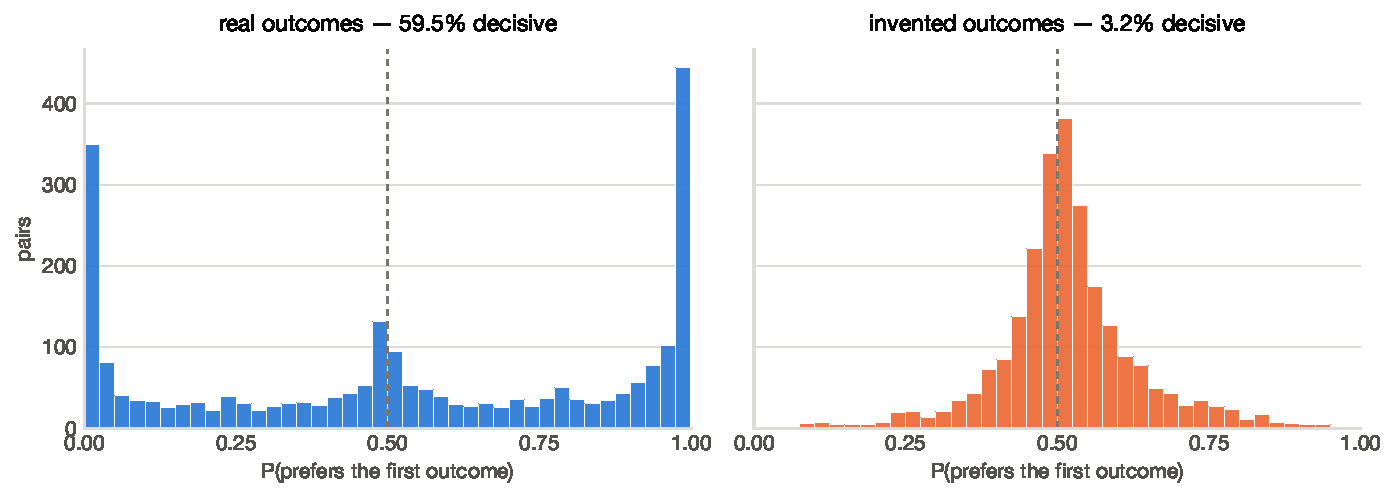
\includegraphics[height=.68\textheight,width=\textwidth,keepaspectratio]{fig3_strength.pdf}
  \end{center}
  \small
  Real outcomes: mass at the edges. Invented: mass at indifference.
  Coherence reads only \emph{which side of 0.5}.
\end{frame}

\begin{frame}{Backup --- persona displacement}
  \begin{center}
    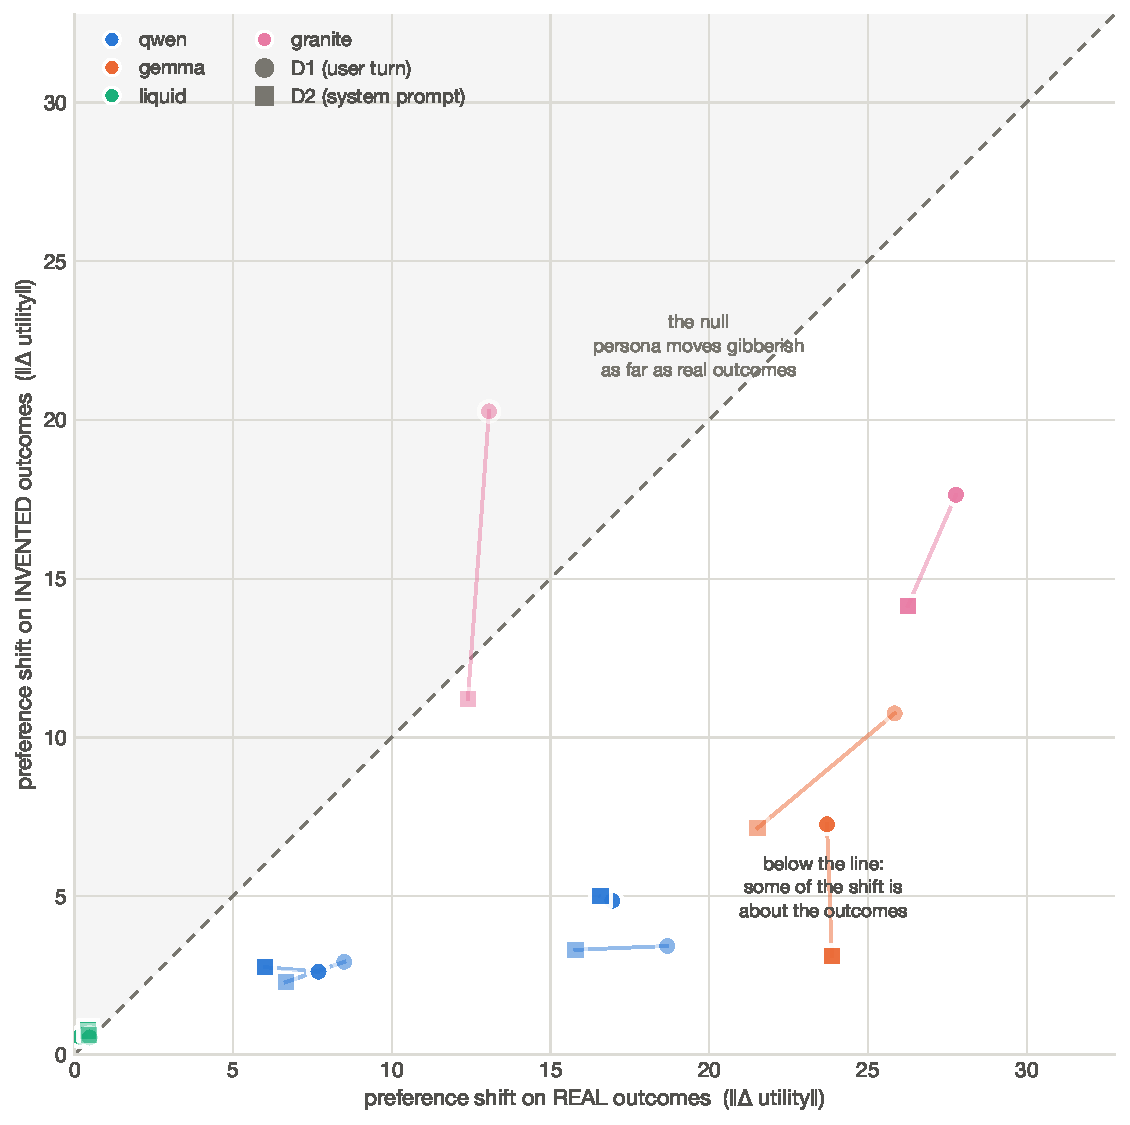
\includegraphics[height=.68\textheight,width=\textwidth,keepaspectratio]{fig5_persona.pdf}
  \end{center}
  \small
  Dashed diagonal is the null. \hl{Below} it = displacement the invented-outcome
  control cannot explain.
\end{frame}

\end{document}
